\documentclass[10pt,a4paper]{article}
\usepackage[utf8x]{inputenc}
\usepackage{ucs}
\usepackage[english]{babel}
\usepackage{amsmath}
\usepackage{amsfonts}
\usepackage{amssymb}
\usepackage{makeidx}
\usepackage{graphicx}
\usepackage{lmodern}
\usepackage{kpfonts}
\usepackage{float}
\usepackage{enumitem}

\usepackage[left=2cm,right=2cm,top=2cm,bottom=2cm]{geometry}

\usepackage{titlesec}

\renewcommand{\o}{\circ}
\newcommand{\qed}{\blacksquare}
\newcommand{\R}{\mathbb{R}}

% elimina newline despues de \section:
\titleformat{\section}[runin]
{\normalfont\large\bfseries}{\thesubsection}{1em}{}      


\headsep17mm
\topmargin-1cm
\hoffset -1.5cm \voffset -1cm \textwidth 17cm \oddsidemargin
1.5cm \evensidemargin 1.5cm \textheight 22.5cm


\setlength\parindent{0cm}

\begin{document}

\vspace{0,3cm}

\begin{center}
{\bf \Large Resoluciones seleccionadas, semana 10}
\end{center}


\vspace{0,3cm}

\section*{1.6.d}\emph{}

\noindent
Esto es falso.
Para construir el contraejemplo podr\'iamos considerar funciones
trigonom\'etricas, que intuitivamente ya manejamos.
Otro ejemplo no trivial es definir una funci\'on
(como ya se hizo anteriormente en el curso)
$[ ] : \mathbb{R}\rightarrow\mathbb{R}$ donde $[x]$ es la distancia
de $x$ al entero mas pr\'oximo.
Es f\'acil probar que esta funci\'on est\'a acotada
($0\leq[x]\leq\frac{1}{2}$), que adem\'as es continua,
y ver que intuitvamente no tiene l\'imite
infinito.


\begin{center}
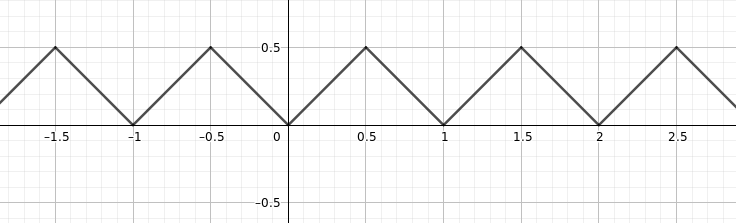
\includegraphics[height=3.5cm]{./imgs/function}
\end{center}




Formalicemos \'esto. Lo haremos en particular para el l\'imite
con $ x \rightarrow +\infty$
pero el otro caso es an\'alogo

\noindent
Observemos que la definici\'on de $\displaystyle{\lim_{x\rightarrow +\infty}
  [x]= l}$.
es que dado $\epsilon > 0$ podemos encontrar
$K\in\mathbb{R}$ tal que si $x > K$ entonces $|[x]-l|<\epsilon$.
M\'as precisamente:
$$
\forall \epsilon>0, \exists K\in\mathbb{R} \: : \: \forall x>K, \: |[x]-l|<
\epsilon
$$

\noindent
La {\bf negaci\'on} de esta proposici\'on es 

$$
\displaystyle{
\exists \epsilon>0 \: / \:
\forall K\in\mathbb{R}, \: \exists x>K \text{ con }
\left|[x]-l\right|>\epsilon}
$$

\noindent
Es decir, podemos dar un $\epsilon$ tal que sin importar que tan grande sea
$K$, podemos encontrar $x>K$ con $|[x]-l|>\epsilon$.

\noindent
Tomamos $\epsilon=\frac{1}{4}$. Dado $K$, elegimos $x_0\in\mathbb{N}$ con
$x_0>K$ (Podemos porque ya demostramos que los naturales no est\'an acotados).

\noindent
Tomamos $x_1 = x_0 + \frac{1}{2}$.

$$
  |[x_0] - l| + |[x_1] - l|
= |[x_0] - l| + |l - [x_1]| \geq |[x_0] - [x_1]| = \frac{1}{2}
$$

Donde aplicamos la desigualdad triangular.

\noindent
Pero entonces tenemos dos reales positivos que suman $\frac{1}{2}$
($|[x_0] - l|$ y $|[x_1] - l|$),
por lo que
uno de ellos debe valer por lo menos $\frac{1}{4}$. Supongamos que es
$x_0$ sin perder generalidad. As\'i encontramos $x_0$ tal que
$|[x_1] - l| > \epsilon$ 


\section*{1.6.h}\emph{}

Falso. Consideramos $\displaystyle{f(x) = \frac{1}{x^2}}$.
La funci\'on no tiene m\'aximo (no est\'a acotada).
Para probarlo formalmente, consideremos $y_0 > 0$
tan grande como se quiera, tomando $x$ tal que
$\displaystyle{ 0 < x < \sqrt{\frac{1}{y_0}}}$
basta para encontrar una imagen mayor:

$$
x < \sqrt{\frac{1}{y_0}} \implies x^2
< \frac{1}{y_0} \iff y_0 < \frac{1}{x^2} = f(x)
$$


Tampoco tiene m\'inimo. De hecho $Im(f) = \left( 0, + \infty\right)$.
Para probarlo observar que $\displaystyle{\frac{1}{x^2}}$
es siempre positivo,
por lo que $im(f)\subseteq \left( 0, + \infty\right)$. Y dado
$y\in \left( 0, + \infty\right)$ construimos una preimagen
$\sqrt{\frac{1}{y}}$ por lo que $\left( 0, + \infty\right)
\subseteq im(f)$, probando as\'i la doble inclusi\'on
y por tanto la igualdad.



\end{document}
